\documentclass[11pt,letterpaper]{article}

% \documentclass{article}
%    \usepackage{amsmath}
%    \usepackage{amssymb}
%    \usepackage{amsfonts}
%    \usepackage{graphicx}
%    \usepackage[mathscr]{euscript}
%    %\usepackage{bbm}
%    \usepackage[margin=1.0in]{geometry}
%    \usepackage{hyperref}
%    \usepackage{comment}
%    %\usepackage{todonotes}

%    %\usepackage{simplewick}
%    \usepackage{slashed}
%    %\usepackage{undertildeMod}

%    %\usepackage{feynmp-auto}
%    %\usepackage{youngtab}
%    %\usepackage[vcentermath]{youngtab}

%\usepackage{tikz}

%    \usepackage{enumitem}

    \newcommand{\vectsym}[1]{ \vec{#1} }
    %\newcommand{\vectsym}[1]{ \overline{#1} }
    %\newcommand{\vect}[1]{\vectsym{\boldsymbol{#1}}}
%    \newcommand{\vect}[1]{\boldsymbol{#1}}
    \newcommand{\vect}[1]{\vectsym{#1}}

    \newcommand{\udd}[2][]{{{\mathrm{d}^{#1}} #2}}
    \newcommand{\ud}[2][]{{ \, \udd[#1]{#2} \,}}
    \newcommand{\dd}[3][]{\frac{\udd{^{#1} #2 }}{\udd{ {#3}^{#1} }}}
    \newcommand{\uDD}[2][]{{{\mathcal{D}^{#1}} #2}}
    \newcommand{\uD}[2][]{{ \, \uDD[#1]{#2} \,}}
    \newcommand{\fdd}[3][]{{  \frac{ {\delta^{#1}}#2}{\delta #3} }}
    \newcommand{\vdd}[3][]{{ \fdd[#1]{#2}{#3}  }}
    %\newcommand{\pdd}[2]{ \frac{ \partial{#1} }{ \partial{#2} } }
    \newcommand{\limint}[2]{ \int\limits_{#1}^{#2} }
    \newcommand{\limintf}[4]{\limint{#1}{#2}\frac{#3}{#4}}
    \newcommand{\limintd}[3]{ \int\limits_{#1}^{#2}{\udd{#3}\,} }
    %\newcommand{\intd}[1]{ \int{\udd{#1}} }
    \newcommand{\intd}[2][]{ \int{\udd[#1]{#2}\,} }
    \newcommand{\intD}[2][]{ \int{\uDD[#1]{#2}\,} }
    \newcommand{\intdf}[3][]{\int\frac{\ud[#1]{#2}}{#3}}
    \newcommand{\intdff}[4][]{\int\frac{\ud[#1]{#2}#3}{#4}}
    \newcommand{\limintdf}[5][]{\limint{#2}{#3}\frac{\ud[#1]{#4}}{#5}}
    \newcommand{\limintdff}[6][]{\limint{#2}{#3}\frac{\ud[#1]{#4}#5}{#6}}

    \newcommand{\unit}[1]{\,\widehat{ \boldsymbol{#1} }}
    \newcommand{\paren}[1]{{\left( #1 \right)}}
    \newcommand{\bparen}[1]{\Bigl( #1 \Bigr)}
    \newcommand{\bbparen}[1]{\Biggl( #1 \Biggr)}
    \newcommand{\brac}[1]{\left[ #1 \right]}
    \newcommand{\bbrac}[1]{\Bigl[ #1 \Bigr]}
    \newcommand{\bbbrac}[1]{\Biggl[ #1 \Biggr]}
    \newcommand{\cbrace}[1]{{ \left\{ #1 \right\} }}
    \newcommand{\bcbrace}[1]{{ \Bigl\{ #1 \Bigr\} }}
    \newcommand{\bmat}[1]{  \begin{bmatrix}  #1  \end{bmatrix}   }
    \newcommand{\pmat}[1]{  \begin{pmatrix}  #1  \end{pmatrix}   }
    %\newcommand{\inv}[1]{\frac{1}{ #1 } }
    \newcommand{\ddsq}[2]{\frac{\udd^2}{\udd{ #2 }^2} #1 }
    \newcommand{\nline}[1]{\noindent\textbf{ #1 }}
    \newcommand{\nprob}[2]{\nline{ #1 } \begin{align*} #2  \end{align*} }
    \newcommand{\neqs}[2][*]{\begin{align#1} #2 \end{align#1}}
    \newcommand{\abs}[1]{\left| #1 \right|}
    \newcommand{\flux}[0]{\Phi}
    \newcommand{\del}[0]{\nabla}
    \newcommand{\vdel}[0]{\vect{\del}}
    \newcommand{\eval}[2]{\biggl|_{#1}^{#2}\biggr. }
    \newcommand{\smeval}[2]{\Bigl|^{#1}_{#2}\Bigr. }
    \newcommand{\pd}[1]{\partial #1}
    \newcommand{\pdd}[3][]{\frac{\pd{^{#1} #2 }}{\pd{ {#3}
    %^{#1}
    }}}
    \newcommand{\ang}[1]{\left\langle #1 \right\rangle}
    \newcommand{\expon}[1]{ \,\mathrm{e}^{ #1 } }
    \newcommand{\emf}[0]{\varepsilon}

    \newcommand{\bfrac}[2]{ \brac{\frac{ #1 }{ #2 }} }
    \newcommand{\pfrac}[2]{ \paren{\frac{ #1 }{ #2 }} }
    \newcommand{\ptfrac}[2]{ \paren{\tfrac{ #1 }{ #2 }} }
    \newcommand{\vud}[2][]{ \ud{#1\vect{ #2 }} }

    \newcommand{\ee}[1]{\times10^{#1}}
    \newcommand{\un}[1]{\,\mathrm{ #1 }\,}
    \newcommand{\ans}[3]{\, #1 \ee{#2} \un{#3} }
    \newcommand{\qty}[3]{\paren{\, #1 \ee{#2} \un{#3} }}
    \newcommand{\smqty}[2]{\paren{\, #1 \un{#2} }}
    \newcommand{\smans}[2]{\, #1 \un{#2} }

    \newcommand{\basis}[1]{ \,\unit{\mathrm{e}}_{ #1 } }
    \newcommand{\q}[1]{q_{#1}}
    \newcommand{\bq}[1]{\,\unit{\mathrm{q}}_{#1}}
    \newcommand{\be}[1]{\basis{#1}}
    \newcommand{\bbe}[2]{\be{#1}\be{#2}}
    \newcommand{\bep}[1]{\be{#1}'}
    \newcommand{\vectc}[3]{ \vectcc{#1}{+#2}{+#3} }
    \newcommand{\vectcc}[3]{#1 \basis{x} #2 \basis{y} #3 \basis{z} }
    \newcommand{\tensor}[1]{#1}
    \newcommand{\tp}[0]{\mathrm{T}}%transpose
    \newcommand{\infsum}[1]{ \sum_{n=0}^{\infty}{#1} }
    \newcommand{\dualsum}[1]{\infsum{}\sum_{k=0}^{n}{#1}}
    \newcommand{\qeq}[0]{\overset{?}{=}}
    \newcommand{\res}[0]{\,\mathrm{res}}
    \newcommand{\resw}[1]{\res\paren{w,#1}}
    \newcommand{\Four}[1]{\mathscr{F}\left\{ #1 \right\}}
    \newcommand{\invFour}[1]{\mathscr{F}^{-1}\left\{ #1 \right\}}
    \newcommand{\Heav}[0]{\,\mathrm{H}}
    \newcommand{\heav}[0]{\Heav}
    \newcommand{\delt}[0]{\,\delta}
    \newcommand{\infint}[0]{\int_{-\infty}^{\infty}}
    \newcommand{\infintd}[1]{\infint\ud{#1}}
    \newcommand{\conv}[0]{\otimes}
    \newcommand{\scr}[1]{\mathscr{#1}}
    \newcommand{\Lap}[1]{\mathscr{L}\left\{ #1 \right\}}
    \newcommand{\invLap}[1]{\mathscr{L}^{-1}\left\{ #1 \right\}}
    \newcommand{\iif}{\quad \mathrm{if}\,}

    \newcommand{\pw}[2][cc]{\left\{ \begin{array}{#1} #2 \end{array} \right. }

    \newcommand{\pcos}[1]{\cos{\paren{#1}}}
    \newcommand{\psin}[1]{\sin{\paren{#1}}}

    \newcommand{\uu}[1]{\underline{#1}}
    \newcommand{\eq}[2][\notag]{\begin{equation}#1 #2 \end{equation}}
    \newcommand{\enum}[1]{\begin{enumerate} #1 \end{enumerate} }
    \newcommand{\bitem}[1]{\item[\textbf{#1}]}
    \newcommand{\bbitem}[2]{\item[\textbf{#1}] (#2)\,}

    \newcommand{\ffrac}[3][]{{ #1{\frac{#2}{#3}} }}
    \newcommand{\poissonbrac}[1]{ {\left\{ #1 \right\}} }
    \newcommand{\bars}[1]{{\left| #1 \right|}}
    \newcommand{\detmat}[1]{\begin{vmatrix} #1 \end{vmatrix}}
    \newcommand{\qtq}{\quad\to\quad}
    \newcommand{\qTq}{\quad\implies\quad}
    \newcommand{\opdot}[1]{\overset{\scriptscriptstyle \circ}{#1}}
    \newcommand{\opddot}[1]{\overset{\circ\circ}{#1}}

	\newcommand{\enumb}[1][]{\begin{enumerate}[#1]}
    \newcommand{\enume}{\end{enumerate}}

    \newcommand{\rr}{\vect{r}}
    \newcommand{\R}{\mathbb{R}}
    \newcommand{\Z}{\mathbb{Z}}

    \newcommand{\upperlower}[3]{{ {#1}^{#2}_{\phantom{2}#3} }}
    %\newcommand{\ul}[3]{\upperlower{#1}{#2}{#3}}
    \newcommand{\lowerupper}[3]{{ {#1}_{#2}^{\phantom{2}#3} }}
    %\newcommand{\lu}[3]{\lowerupper{#1}{#2}{#3}}

    \newcommand{\ket}[1]{{ \left | #1 \right \rangle }}
    \newcommand{\bra}[1]{{ \left \langle #1 \right | }}
    \newcommand{\bk}[2]{{ \left \langle #1 \middle | #2 \right \rangle }}
    \newcommand{\bok}[3]{{ \left \langle #1 \middle | #2 \middle | #3 \right \rangle }}
    \newcommand{\bo}[2]{{ \left \langle #1 \middle | #2 \right .}}
    \newcommand{\ok}[2]{{ \left . #1 \middle | #2 \right \rangle}}
    \newcommand{\kb}[2]{{ \ket{#1}\bra{#2} }}

    \renewcommand{\a}[1][\vphantom{\dagger}]{{a^{#1}}}
    \newcommand{\ad}{\a[\dagger]}
    \newcommand{\kk}{{k\vphantom{k'}}}
    \newcommand{\kp}{{k'}}
    \newcommand{\kpp}{{k''}}
    \newcommand{\comm}[2]{\brac{\,#1\,,\,#2\,}}
    \newcommand{\acomm}[2]{\cbrace{\,#1\,,\,#2\,}}
    \renewcommand{\L}{\scr{L}}
    \newcommand{\inv}{^{-1}}
    \newcommand{\norder}[1]{\,: #1 :\,}
    \newcommand{\obar}[1]{{ \overline{#1} }}
    \newcommand{\wick}[6][1]{{ \contraction[#1 ex]{#2}{#3}{#4}{#5} #2#3#4#5#6}}
    \newcommand{\sq}{^{\,2}}
    \newcommand{\fcn}[1]{{\,\mathrm{#1}\,}}
    \newcommand{\op}[1]{\widehat{#1}}
    \newcommand{\tr}{\fcn{tr}}
    \newcommand{\Tr}{\fcn{Tr}}
    \newcommand{\T}{\fcn{T}}

    \newcommand{\lra}{\leftrightarrow}
    \newcommand{\nothing}[1]{}
    \newcommand{\half}[1][1]{ {\frac{#1}{2}} }
    \newcommand{\thalf}[1][1]{ {\tfrac{#1}{2}} }
    \newcommand{\id}{ {\mathbf{1}} }
    \newcommand{\sigmab}{ {\bar{\sigma}} }
    \newcommand{\dg}{ {\dagger} }
    \newcommand{\pdg}{ {\vphantom{\dagger}} }
    \newcommand{\gr}[1]{ {\mathrm{#1}} }

    %\DeclareSymbolFont{bbold}{U}{bbold}{m}{n}
    %\DeclareSymbolFontAlphabet{\mathbbold}{bbold}

    \newcommand{\kd}[2]{{ \delta^{#1}_{#2}}}
    \newcommand{\kdu}[1]{{ \delta^{#1}}}
%    \newcommand{\Sl}[1]{{{ S_{#1}}}
%    \newcommand{\Su}[1]{{{ S^{#1}}}
%    \newcommand{\Smat}[4]{{{ (S_{#1#2})^{#3#4}}}
%    \newcommand{\kdg}[4]{{{ \kd{#3}{#1}\kd{#4}{#2}}}
%    \newcommand{\kdgg}[4]{{{ \kd{#4}{#1}\kd{#3}{#2}}}
%    \newcommand{\Smatd}[4]{{{ \kdg{#1}{#2}{#3}{#4}-\kdgg{#1}{#2}{#3}{#4}}}
%    \newcommand{\Smatdp}[4]{{{ \big(\Smatd{#1}{#2}{#3}{#4}\big)}}
%    \newcommand{\g}[1]{g_{#1}}
%    \newcommand{\gu}[1]{g^{#1}}
%····
    \newcommand{\ub}{\overline{u}}
    \newcommand{\vb}{\overline{v}}
    \newcommand{\gv}{\gamma^5}
    \newcommand{\gm}[1]{{\gamma^{#1} }}
%    \newcommand{\Tr}[1]{\,\mathrm{Tr}\brac{#1}}
    \newcommand{\ps}{\slashed{p}}
    \newcommand{\ks}{\slashed{k}}
    \newcommand{\pds}{\slashed{\pd}}
    \newcommand{\psib}{\bar{\psi}}

%    \newcommand{\ul}[3][]{#1^{#2\phantom{#3}}_{\phantom{#2}#3} }
    \newcommand{\ulul}[5][]{#1^{#2\phantom{#3}#4\phantom{#5}}
                            _{\phantom{#2}#3\phantom{#4}#5} }
    \newcommand{\symindBinU}[5]{ {#1}^{#2#3}{#1}^{#4#5} 
                                    + {#1}^{#2#4}{#1}^{#3#5}
                                    + {#1}^{#2#5}{#1}^{#3#4} }
    \newcommand{\symindBinL}[5]{ {#1}_{#2#3}{#1}_{#4#5} 
                                    + {#1}_{#2#4}{#1}_{#3#5}
                                    + {#1}_{#2#5}{#1}_{#3#4} }
    \newcommand{\gindBinU}[5]{ {#1}^{#2#3}{#1}^{#4#5} 
                                    - {#1}^{#2#4}{#1}^{#3#5}
                                    + {#1}^{#2#5}{#1}^{#3#4} }
    \newcommand{\gind}[4]{\gindBinU{g}{#1}{#2}{#3}{#4} }
    \newcommand{\tot}{\leftrightarrow}
    \newcommand{\diag}{\fcn{diag}}
    \newcommand{\itemb}{\begin{itemize}}
    \newcommand{\iteme}{\end{itemize}}

    \newcommand{\newQuestion}[2]{ \section*{Question #1 \textnormal{: #2 } } }
    \newcommand{\hc}{ {\text{h.c.}} }
    \newcommand{\ptext}[1]{\paren{\text{#1}}}

    \newcommand{\set}[1]{ \cbrace{#1} }
    \newcommand{\lie}[3][]{ {{\mathrm{#2}}_{#1}\paren{#3} } }

    \newcommand{\lag}{ {\mathcal{L}} }
    \newcommand{\Lag}{ \lag }
    \newcommand{\amp}[1][M]{ {\mathcal{#1}} }
    \newcommand{\Amp}[1][M]{ \amp[#1] }

    \newcommand{\p}{\vect{p}}

    \newcommand{\fig}[2][]{
	    \begin{figure}[#1]\begin{center}
		    #2
	    \end{center}\end{figure}
    }



% filename: PhysMan.tex

%% FOR Sans Serif UNCOMMENT THE FOLLOWING TWO LINES
%\usepackage[T1]{fontenc}
%\renewcommand*\familydefault{\sfdefault} %% Only if the base font of the document is to be sans serif
%% (To get normal Serif font again, comment the two lines)


%----------------------------------------------------------------
% Attempts at changing the font to sans serif style
%----------------------------------------------------------------

% http://www.tug.dk/FontCatalogue/sansseriffonts.html

%%\usepackage[light,math]{iwona}
%%\usepackage[T1]{fontenc}

%%\usepackage{cmbright}
%%\usepackage[T1]{fontenc}

% Works:
%\usepackage[T1]{fontenc}
%\renewcommand*\familydefault{\sfdefault} %% Only if the base font of the document is to be sans serif

%%\usepackage[default]{sourcesanspro}
%%\usepackage[T1]{fontenc}



%----------------------------------------------------------------
% Other style options
%----------------------------------------------------------------

\usepackage{fullpage}
\usepackage{graphicx}
\usepackage{amsmath}
\usepackage{amssymb} % Math symbols such as \boldsymbol

\usepackage{fancyhdr}
\pagestyle{fancy}
%\fancyfoot[C]{\thepage}
\usepackage[
%  margin=2.5cm,
  left=2.5cm, right=2.5cm,
  top=2cm, bottom=2cm,
  includefoot,
  footskip=30pt,
  headsep=1.25cm % Seperate header and main body by
		% headsep -- prevents first line from overlaying on top of header
]{geometry}

\usepackage[noams,squaren,Gray]{SIunits} % Standardizes quantity and SI unit spacing
\usepackage{soul} % for an underline macro that wraps
 \setul{0.2ex}{.4pt}% underline 0.2ex below contents
\usepackage{enumitem} % for enumerate options
\usepackage{verbatim} % Allows display of almost any sequence of symbols, printed in typewriter font; and provides comment environment
\usepackage[obeyspaces,spaces]{url} % Same as verbatim but allows line breaks and spaces
\usepackage{parskip}
 \setlength{\parindent}{0em}
 \setlength{\parskip}{2.2ex}

%\usepackage[compact]{titlesec}
%\titlespacing{\section}{0pt}{*1ex}{*0.5ex}
%\titlespacing{\subsection}{0pt}{*0}{*0}
%\titlespacing{\subsubsection}{0pt}{*0}{*0}
\usepackage{titlesec}
\titlespacing{\subsection}{0pt}{*2.5}{*0.1}



%----------------------------------------------------------------
% Macros
%----------------------------------------------------------------

% Scientific Notation and Units
% =============================

% scientific notation without units
\providecommand{\sn}[2]{ {#1} \mkern-1.5mu\times\mkern-3mu 10^{#2} }
% scientific notation with units
\providecommand{\snu}[3]{ \unit{\sn{#1}{#2}}{#3} }

% create compact or ``squished'' lists with sublists:
\newcommand{\squishlist}{
   \vspace{-2.2ex}
   \begin{list}{$\bullet$}
    { \setlength{\itemsep}{0pt}      \setlength{\parsep}{3pt}
      \setlength{\topsep}{3pt}       \setlength{\partopsep}{0pt}
      \setlength{\leftmargin}{1.5em} \setlength{\labelwidth}{1em}
      \setlength{\labelsep}{0.5em} } }
\newcommand{\squishend}{
    \end{list}  }

% struts for spacing in tabulars/tables
\newcommand{\tstrut}{\rule{0pt}{2.5ex}}
\newcommand{\bstrut}{\rule[-1ex]{0pt}{0pt}}
\newcommand{\Tstrut}{\rule{0pt}{2.9ex}}
\newcommand{\Bstrut}{\rule[-1.4ex]{0pt}{0pt}}


\usepackage{todonotes}
%\graphicspath{{../../imgs/6labs/6Alab/6Aexp6/}}
\graphicspath{{../../}}

\begin{document}

\fancyhead[C]{Physics 6A Lab \rule[-1ex]{0pt}{0pt}\(\mid\) Experiment 6}
%\fancyhead[C]{Physics 6A Lab \rule[+1ex]{5pt}{5pt}\(\mid\) Experiment 6}

\vspace{-5ex}
\part*{Overhauled Bicep Lab}

\subsection*{Notes from Allic}
\enumb
\item Main suggestion:  Cut content and make things inquiry-based
\item Just saying at the beginning something like ``This lab will be
	different.  We're expecting you to think about what steps to take,
	rather than just follow a recipe" has a big effect on the students'
	attitudes.  
	[Jared is not surprised by this, though he hadn't thought of doing it.]  
\enume

\subsection*{Warm-up}
\subsubsection*{Meet the apparatus}
In this experiment, you'll attempt to understand torques and rotational
equilibrium using a model of the human arm.

Before we get into equations, take a moment to understand the equipment.  
	Fill in the blanks on the diagram below, from among the following choices:
	upper arm (humerus), elbow, forearm, hand, and biceps muscle.
\todo[inline]{TODO -- Block out the labels in the picture of the apparatus,
	and replace with blanks -- 
	similar to a diagram one might fill in for a biology
	course.  Blanks include 
	upper arm (humerus), elbow, forearm, hand, and biceps muscle.}

\begin{figure}[h!]
	\centering
	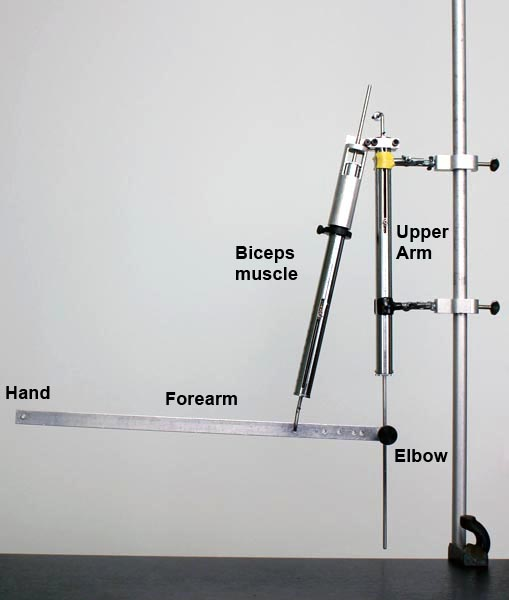
\includegraphics[width=0.6\textwidth]
	{{/imgs/6labs/6Alab/6Aexp6/6a-exp6_fig1_text_fix.jpg}}
\end{figure}

\subsubsection*{Get your head in the game}

Before making use of the apparatus,
let's do a brief warm-up problem concerning \emph{torque}.

\todo[inline]{TODO -- Now include an unrelated warm-up problem dealing with
	static torque.  Possibly take this from UMD open source tutorials,
	or from tutorial books.}

\todo[inline]{Maybe include a section getting students acquainted with the
	torque equation we're attempting to verify (relating bicep force to the
	force on the hand).}

\subsection*{Investigation}

Rather than telling you exactly what to do, 
in this lab we're going to allow you much more freedom to
investigate the physics behind this situation on your own.

\section*{Restart}

\subsection*{Warm up -- meta }
\itemb
	\item Assume students don't know anything about torque
	\item Give activity which guides them through torque
	\item Possibly just take from open source tutorial
	\item Ok, open source tutorial requires them to do experiment that we don't
		have resources set up for (though we could relatively easily set them up)
\iteme

\subsection*{Warm up}
Warm up Problems:
\enumb
	\item Balancing weights on a ruler atop a fulcrum
		\enumb[label=\alph*.]
			\item Two equidistant weights on opposite side of pivot
			\item Double one weight's distance; ask how much weight needs to be
				added and to which side
		\enume
	\item Replace one of the weights with an arbitrary force pointing downward
	\item Replace arbitrary force with a cable at an angle 
		(positioned like bicep)
\enume

Need to figure out how to introduce quantitative relations
\itemb
	\item $\tau \sim rF$ (for orthogonal force)
	\item $\tau \sim rF\sin\theta$
\iteme

\subsection*{Procedure}
We wish to investigate some of the forces involved with weight lifting.
Specifically, we'll examine the situation where you're holding a weight in your
hand, with your forearm being horizontal.
We'll measure the forces experienced by both the biceps muscle
and the upper arm.

If you'd like, imagine yourself as a 
physical therapist or prostetic limb designer,
who wishes to combine physics with some 
general experimental design skills to determine 
some of the forces involved in lifting objects.

** Common sense warning about using reasonable values, 
making sure to keep everything but the thing you're measuring constant, etc.**

** Discussion about which variables are relevant.  Answer -- forces, distances,
angles. **

** Make sure to emphasize that we'll keep the forearm horizontal, 
to simplify things. **

Start by measuring the biceps force $B$ and the upper arm force $A$ 
for some fixed weight $H$ being held in the hand.

Then devise and carry out a procedure for measuring the forces $B$ and $A$ for
different weights $H$.

After taking several measurements (you can choose a number which seems
reasonable), use your data to extrapolate a relationship between the biceps
force $B$ and the weight $H$ in the hand.  
Write a quantitative formula for $B$ as a function of $H$.
\emph{Hint:  In case this terminology is a bit unfamiliar, 
it might help to know that, for example, 
$y(t) = \bparen{10\,\mathrm{m}} +\bparen{4.9\,\mathrm{m/s^2}}\times t^2$ 
is a formula for $y$ as a function of $t$ for a certain physical situation.}
Make sure you specify the units of the quantities.

\todo[inline]{This data-only prediction will probably be cut for the sake of time}
Choose a new value for $H$ -- one that you haven't measured yet,
but that you are able to measure.  
Before you measure $B$, use your model to predict the biceps force $B$ 
for this value of $H$.

** Ideally, first make a rough prediction of $B$ based only on neighboring data
points. **

Now use the apparatus to measure $B$ for this value of $H$.  How does it
compare to the prediction from your model?  
(Calculate the percent deviation.)

\subsubsection*{Extrapolate further}
The model you extrapolated from your data is a good description of the 
force $B$ on this apparatus for this setup.  But what if you change the
apparatus somehow?  For example, consider an apparatus which
is the same as yours, except the forearm bar is longer.
For the same value of the weight $H$ in the hand, 
would the corresponding biceps force $B$ change? 
In fact, it does -- $B$ is larger for a larger value of $R$ 
(assuming all other parameters are left the same).
** Ideally ask them a question, to make sure they pay attention to this part.
**

In reality, you probably want a model of the biceps force that is valid 
beyond your specific biceps setup.  





\end{document}
